\section{Prehľad problematiky}
Digitalizácia najrôznejších aspektov nášho života je prirodzeným prejavom technologického pokroku. Vďaka tomu sa 
pojmy, ako zmiešaná realita, rozšírená realita či virtuálna realita v~priebehu posledných dekád začali stávať neoddeliteľnou súčasťou nášho jazyka. 
Na to, aby sme lepšie porozumeli tomu, čo to zmiešaná realita vlastne je, pokladáme za nevyhnutné venovať niekoľko odstavcov aj zvyšným dvom pojmom.

\subsection{Virtuálna realita}
\begin{quote}\itshape
  The ultimate display would, of course, be a room within which the computer can control the existence of matter. A chair displayed in such a~room 
  would be good enough to sit in. Handcuffs displayed in such a room would be confining, and a~bullet displayed in such a~room would be fatal. 
  With appropriate programming such a display could literally be the Wonderland into which Alice walked \cite{sutherlandUltimateDisplay1965b}.
\end{quote}
Týmito slovami v roku 1965 Ivan Sutherland vo svojom článku \emph{The Ultimate Display} sformuloval ideu, ktorá predstavuje raný popis 
imerzívneho\footnote{Z angl. \emph{immersive} - voľne preložené ako vťahujúci do deja} displeja v dobe, keď vtedajšie zariadenia bežne umožňovali 
zobrazovať rovné čiary, uvažovalo sa, že zobrazovanie kriviek by mohlo byť užitočné a žiadna komerčne dostupná obrazovka nebola schopná vykresliť farbou 
vyplnenú plochu \cite{sutherlandUltimateDisplay1965b}. 

Sutherland vo svojom článku okrem iného zdôrazňuje, že počítačové displeje môžu umožniť zoznámenie sa s pojmami, ktoré nie sú realizovateľné vo fyzickom svete, 
a slúžia ako možnosť nahliadnuť do matematickej krajiny zázrakov \emph{(sic)}. Článok sa zaoberá aj rôznymi vstupnými zariadeniami na interakciu s počítačovými 
displejmi, ako sú klávesnice písacích strojov, svetelné perá, dotykové pero RAND Tabletu\footnote{Jedno z prvých digitálnych zariadení pre kreslenie rukou a prvé, 
ktoré bolo predávané ako ,,low-cost''}, tlačidlá, joysticky a hlasový vstup, pričom zdôrazňuje ich užitočnosť pri interakcii s počítačom. 

Okrem toho sa v článku uvádza potenciálne využitie pohybov svalov a očí na ovládanie počítačov. Poukazuje na to, že hoci súčasné systémy využívajú na ovládanie 
počítača predovšetkým svaly ruky a ramena, existuje možnosť využiť na interakciu aj iné svalové skupiny. 

Článok navyše uvažuje o perspektíve osvojenia si jazyka pohľadov na ovládanie počítača, navrhujúc, že prezentácia na displeji by sa mohla meniť na základe pohybov 
očí používateľa. Táto koncepcia otvára priestor pre vytváranie intuitívnejších a personalizovanejších rozhraní, čo môže viesť k inovatívnym spôsobom interakcie 
s počítačovými systémami.

Krátko potom Sutherland skonštruoval prvý interaktívny systém slúžiaci na zobrazovanie virtuálnej reality, ktorý si vyslúžil priliehavú prezývku 
\emph{Damoklov meč} \cite[5]{schmalstiegAugmentedRealityPrinciples2016}, pozri obr. \ref{sutherland-device}. Trojrozmerný displej s~upevnením na hlavu, ktorý 
Sutherland vo svojej práci \cite{sutherlandHeadmountedThreeDimensional1968} popísal v~roku 1968, pozostával zo špeciálnych okuliarov, 
ktoré na sebe mali upevnené dve miniatúrne obrazovky typu \acrshort{crt} a~boli pevnou súčasťou ramena visiaceho zo stropu miestnosti. 
Okrem zníženia fyzickej záťaže používateľa, ktorá vznikala kvôli hmotnosti zariadenia, toto rameno slúžilo ako mechanický snímač polohy hlavy a~spolu s~ďalším, 
ultrazvukovým snímačom generovalo vstupné údaje pre výpočet rotačnej a~translačnej matice. Tie boli súčasťou operácií nevyhnutných pre dynamické generovanie obrazu. 
Objekty, z~ktorých pozostával výsledný obraz, boli poskladané z~jednoduchých čiar a~vytvárali tzv.~wireframe model.

\begin{figure}[!htbp]
  \centering
  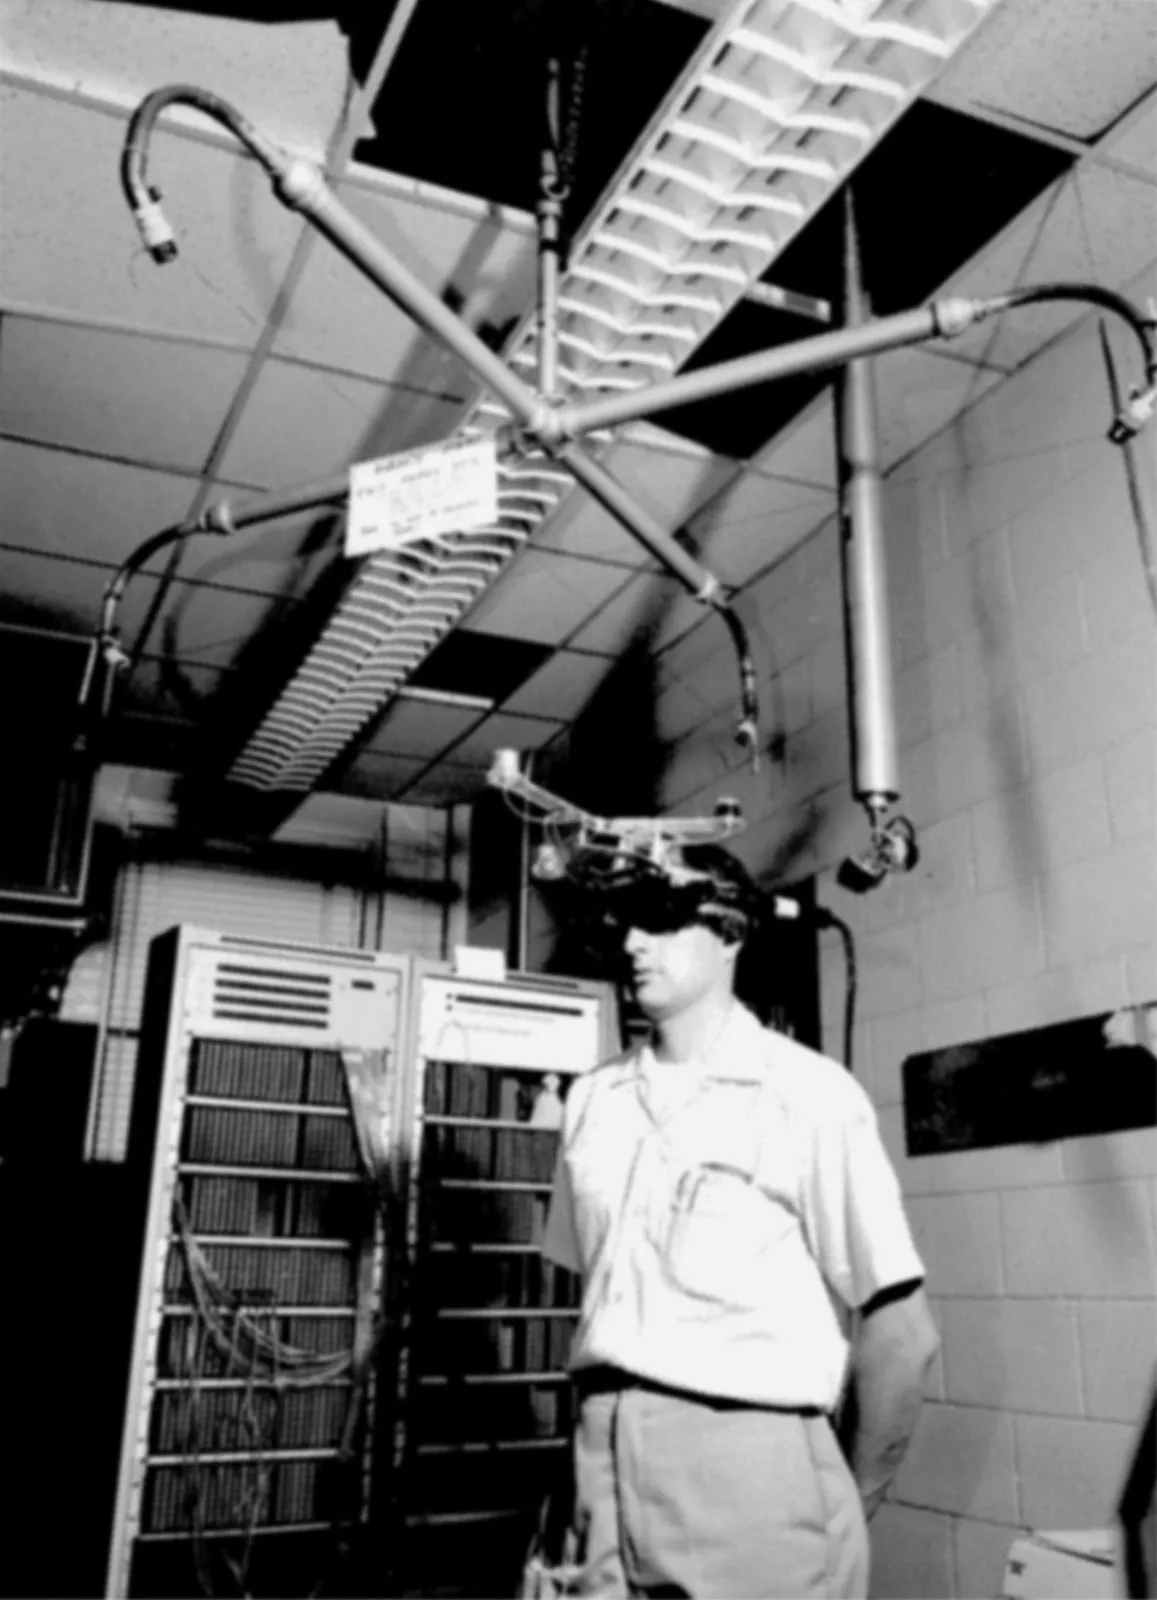
\includegraphics[width=7cm]{img/display-device-Ivan-Sutherland-Harvard-University-1967.jpg}
  \caption{Zobrazovacie zariadenie Ivana Sutherlanda}
  \label{sutherland-device}
\end{figure}	

Sutherlandovo dielo významne prispelo k rozvoju myšlienok a technológií súvisiacimi s~vizualizáciou umelého sveta. Postupom času vzniklo množstvo ďalších 
prototypov rôznorodých systémov, ktoré sa líšili nie len účelom použitia, ale aj spôsobom vzájomnej interakcie s~človekom a~aj tým, či a~ako veľmi bol umelý 
svet prepojený s tým skutočným. Ako príklad uvedieme systém VIDEOPLACE Myrona Kruegera z roku 1985, ktorý kombinuje zosnímanú postavu používateľa s~umelo vytvoreným 
prostredím. Krueger navrhuje využitie tohto systému pre účely telekomunikácie uvádzajúc, že komunikácia medzi priateľmi či obchodnými partnermi nie je 
obmedzená len slovami, a teda je jednoznačne žiadúce, aby geograficky vzdialené osoby mohli zdieľať spoločné virtuálne prostredie 
\cite{kruegerVIDEOPLACEArtificialReality1985}.

Práve Kruegerov systém sprostredkúva to, čo v súčasnej terminológii môžeme označiť ako virtuálnu realitu. Tá prenesie človeka do úplne odlišného prostredia, 
reálne okolie a objekty v ňom nahradí počítačom generovanými, s~cieľom poskytnúť používateľovi intenzívny zážitok z~nového sveta, akoby sa v~ňom skutočne nachádzal
\cite{brighamRealityCheckBasics2017}. 

V deväťdesiatych rokoch minulého storočia bola snaha o rozšírenie zariadení pre virtuálnu realitu medzi bežných spotrebiteľov. Tieto zariadenia však boli cenovo
nedostupné a~spôsobovali používateľom nevoľnosť. Príčinou nevoľnosti bol nesúlad medzi zrakovým a vestibulárnym vnemom; ten bol spôsobený vysokou latenciou medzi pohybom 
hlavy používateľa a~reakciou VR zariadenia na tento pohyb prekreslením virtuálnej scény. 

Prelom nastal až v roku 2014, keď Palmer Luckey, 
zakladateľ spoločnosti Oculus, objavil spôsob, ako znížiť dobu trvania vyhodnocovania polohy hlavy za použitia gyroskopu, akcelerometra a magnetometra. 
Tento úspech opäť naštartoval záujem o túto technologickú oblasť \cite{brighamRealityCheckBasics2017}. V súčasnosti medzi najrozšírenejšie zariadenia patria Oculus Rift S,
HTC Vive Pro, HTC Vive Cosmos, Valve Index a Samsung HMD Odyssey+ \cite{angelovModernVirtualReality2020}. Ďalšou z možností, ktorú propagujú výrobcovia, ako Samsung, Google
a LG, je použitie smartfónu ako displeja vo VR headsete, čo predstavuje cenovo dostupnú alternatívu. Ako príklad uvádzame Samsung Gear VR, ktorý je kompatibilný
s~akýmkoľvek modelom Samsung Galaxy; ďalší príklad je dnes už nepodporovaný Google Cardboard a Google Daydream. 

\subsection{Rozšírená realita}
Podľa výskumu popísaného v článku \cite{speicherWhatMixedReality2019a} definícia rozšírenej reality nie je ani zďaleka tak jednoznačná, ako v prípade virtuálnej reality. 
Jeho autori položili desiatim osobám, ktoré sa zaoberajú virtuálnou a rozšírenou realitou v komerčnej a akademickej sfére, súbor šestnástich otázok, ktoré boli 
navrhnuté tak, aby odhalili rozdiely vo vnímaní toho, čo je virtuálna, rozšírená a zmiešaná realita. Autori uvádzajú, že respondenti sa nezhodovali pri vymenovávaní
relevantných charakteristík rozšírenej reality. Niektorí za rozšírenú realitu pokladajú aj jednoduchú vrstvu\footnote{pôvodne použitý angl. termín \emph{overlay}} 
s~kontextuálnymi informáciami, zatiaľ čo ostatní explicitne uvádzali interakciu s~reálnym prostredím a prekrývanie skutočných objektov počítačom generovanými 
ako jej súčasť.

Chen a Xue uvádzajú, že typický \acrshort{ar} systém musí spĺňať tri podmienky: musí umožňovať interakciu medzi reálnym a virtuálnym obsahom, dokáže v reálnom čase 
prekrývať reálne objekty virtuálnymi, a musí pracovať v trojrozmernom priestore. Takáto funkcionalita vyžaduje použitie rôznych techník sledovania, zobrazovania a
interakcie \cite{chenRenaissanceAugmentedReality2022}.

Techniky sledovania sú používané na zaznamenávanie a overovanie pozície a orientácie používateľov. Zohrávajú dôležitú úlohu pri zosúladení polohy reálnych a virtuálnych
objektov. Pozíciu a orientáciu je možné zisťovať pomocou metód spracovania obrazu, za použitia rozličných senzorov, či kombináciou oboch spôsobov.

Zobrazovacie techniky spájajú virtuálny obsah a reálne prostredie a zobrazujú oboje naraz. V praxi sa uplatnili tri spôsoby zobrazovania: pomocou ručného zariadenia 
(\emph{handheld display}) - napr. smartfón alebo tablet, pomocou náhlavného zariadenia (\emph{headmounted-display}) a za použitia projekcie na povrch reálneho objektu 
(\emph{projection-based display}).

Interakčné techniky zabezpečujú intuitívne používateľské prostredie a adekvátne reakcie systému. Používateľské vstupy pritom môžu byť vo forme gest, hlasových povelov,
prípadne je možné použiť reálny objekt ako ovládací prvok \cite{chenRenaissanceAugmentedReality2022}.

Pomerne známym zástupcom zariadení pre rozšírenú realitu je zariadenie od spoločnosti Google s~názvom Google Glass. Zariadenie v~tvare bežných 
okuliarov, dostupné len počas pomerne krátkeho obdobia (2013 - 2015) \cite{brighamRealityCheckBasics2017} dokázalo používateľovi zobrazovat informácie na malom displeji tesne
nad pravým okom. 

\subsection{Zmiešaná realita}
Zmiešaná realita je najmenej preskúmaný typ umelej reality, pretože je spomedzi trojice \acrshort{vr}, \acrshort{ar} a \acrshort{mr} najmladší. Podobne, ako v prípade
rozšírenej reality, ani tu nejestvuje úplna zhoda v definícii. 

Podľa \cite{speicherWhatMixedReality2019a} existuje šesť spôsobov chápania \acrshort{mr}; ich názvy ponechávame v pôvodnom znení:
\begin{itemize}
  \item \emph{Continuum}
  \item \emph{Synonym}
  \item \emph{Collaboration}
  \item \emph{Combination}
  \item \emph{Alignment}
  \item \emph{Strong \acrshort{ar}}
\end{itemize}

\noindent Vymenované spôsoby chápania \acrshort{mr} sú vysvetlené v nasledujúcich podkapitolách.

\subsubsection*{Continuum}
\acrshort{mr} je chápané v súlade s RV kontinuom\footnote{Reality-Virtuality Continuum}, ktoré je znázornené na obrázku č. \ref{rv-continuum}. V tomto prípade \acrshort{mr}
predstavuje kombináciu reálnych a virtuálnych objektov v rámci spektra medzi úplne reálnym a úplne virtuálnym svetom. To znamená, že \acrshort{mr} môže pozostávať z~
prevažne skutočného sveta s nejakými virtuálnymi objektmi, alebo môže pozostávať z prevažne virtuálneho sveta za prítomnosti nejakých reálnych predmetov. V rámci tohto
kontextu možno chápať \acrshort{vr}, ktoré je na okraji spektra, ako súčasť \acrshort{mr}.

\begin{figure}[!htbp]
  \centering
  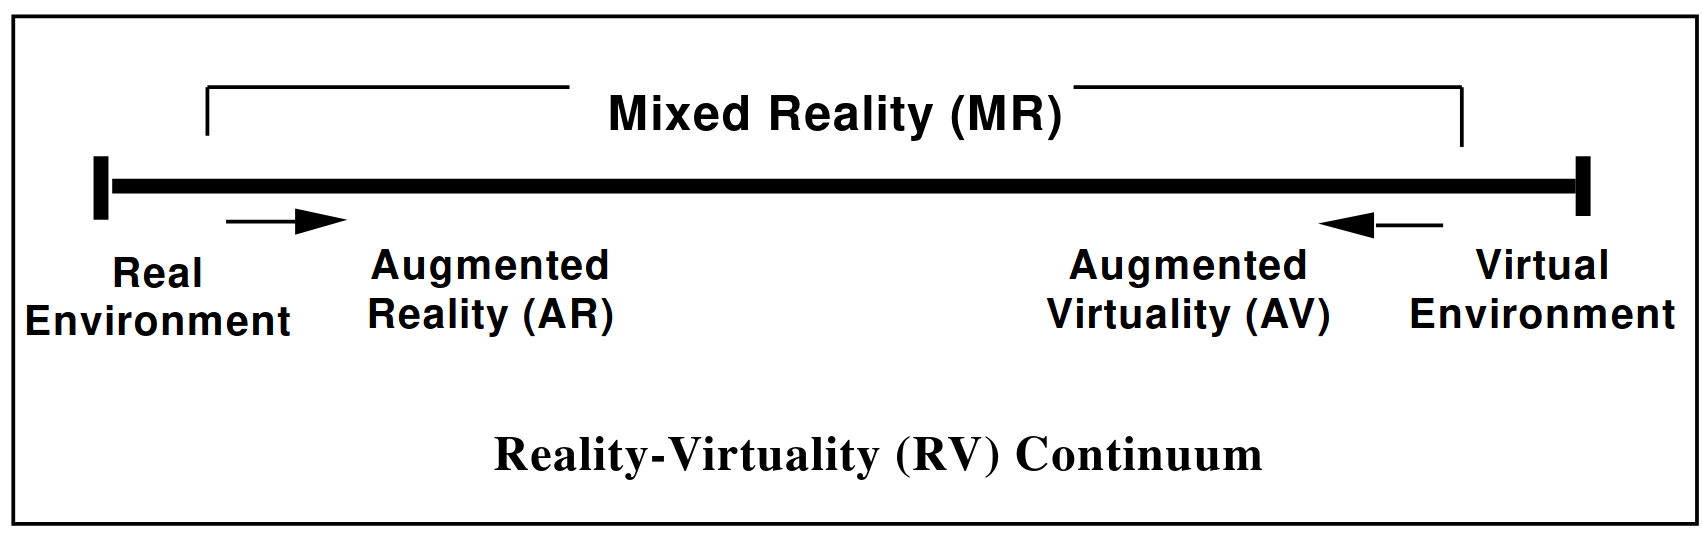
\includegraphics[width=12cm]{img/continuum.png}
  \caption{Zjednodušená reprezentácia RV kontinua \cite{milgramAugmentedRealityClass1995}.}
  \label{rv-continuum}
\end{figure}	

\subsubsection*{Synonym}
V mnohých článkoch, ktoré autori \cite{speicherWhatMixedReality2019a} skúmali, sa používalo \acrshort{mr} ako synonymum pre \acrshort{ar}. To znamená, že tieto pojmy sa 
navzájom zamieňali; \acrshort{mr} bolo použité na označenie systému, ktorý jednoznačne spadal pod \acrshort{ar}, alebo bola použitá definícia \acrshort{ar} na popísanie toho,
čo niektorí autori skúmaných článkov chápali pod pojmom \acrshort{mr}.

\subsubsection*{Collaboration}
Ďalší pohľad vníma \acrshort{mr} ako druh spolupráce. V tomto prípade \acrshort{mr} predstavuje interakciu medzi rôznymi používateľmi \acrshort{ar} a \acrshort{vr}, ktorí
sa nemusia spoločne nachádzať v jednom priestore. Súčasťou tohto typu \acrshort{mr} je rekonštrukcia prostredia, v ktorom sa nachádza používateľ \acrshort{ar}, pre druhého
používateľa prostredníctvom \acrshort{vr}.

\subsubsection*{Combination}
V tomto prípade je \acrshort{mr} chápané ako kombinácia \acrshort{ar} a \acrshort{vr} v zmysle systému, ktorý využíva oddelené časti postavené na \acrshort{vr}, respektíve
\acrshort{ar}. Hoci tieto časti medzi sebou dokážu interagovať, nie sú navzájom pevne prepojené; systém prípadne dokáže podľa potreby prepínať medzi \acrshort{ar} a
\acrshort{vr}. Autori \cite{speicherWhatMixedReality2019a} uvádzajú ako príklad aplikáciu Pokémon GO, kde samotné chytanie Pokémonov je realizované v \acrshort{ar}, zatiaľ čo 
prehľad mapy je plne virtuálny.

\subsubsection*{Alignment}
\acrshort{mr} ako zarovnanie prostredí\footnote{z angl. \emph{alignment of environments}, súosovosť} predstavuje synchronizáciu medzi skutočným a virtuálnym prostredím.
Takýto systém kombinuje virtuálne a skutočné prvky, vďaka čomu tu nájdeme čiastočný prienik s \emph{Combination}, ale prostredia samotné nemusia nutne byť \acrshort{ar}
a \acrshort{vr}. Podobnosť jestvuje aj s \emph{Collaboration}, ale bez prítomnosti aspektu spolupráce a bez toho, aby boli prostredia fyzicky oddelené. Ako príklad sa 
uvádza systém prenášajúci pohyb človeka v reálnom svete do plne imerzívneho virtuálneho prostredia prostredníctvom zariadenia Leap Motion Controller.

\subsubsection*{Strong \acrshort{ar}}
Posledný pohľad na túto problematiku chápe \acrshort{mr} ako \emph{silnejšiu} verziu \acrshort{ar}. Zmiešaná realita je tu charakterizovaná pokročilým vnímaním prostredia
a pokročilými interakciami medzi používateľom a virtuálnymi objektmi, ako aj medzi virtuálnymi objektmi a prostredím. To vytvára predpoklad, že \acrshort{mr} závisí
na konkrétnom hardvéri alebo zariadení, ktoré dokáže poskytnúť požadovanú funkcionalitu. Taktiež sa predpokladá, že \emph{obyčajné} \acrshort{ar} nemá takéto schopnosti,
a tým pádom je \acrshort{mr} evolúciou \acrshort{ar}. \\\\
\noindent
O niečo jednoduchší pohľad na problematiku ponúka Brigham \cite{brighamRealityCheckBasics2017}. Zmiešaná realita (MR) sa opisuje ako spojenie fyzického a virtuálneho sveta, ktoré 
vytvára nové prostredia, v ktorých fyzické a virtuálne objekty koexistujú a interagujú v reálnom čase. MR kombinuje hlavné črty AR aj VR. Umožňuje používateľom vidieť a komunikovať s 
prvkami reálneho aj virtuálneho sveta, ktoré sú uveriteľné a responzívne. Ak je napríklad v MR prostredí virtuálny objekt umiestnený pod skutočným stolom, 
používateľ sa musí zohnúť, aby ho videl, rovnako ako v prípade skutočného objektu. Táto integrácia virtuálnych prvkov do reálneho sveta v MR umožňuje viac imerzívny zážitok v porovnaní 
s AR, kde sú reálne objekty jednoducho prekryté virtuálnymi prvkami bez akejkoľvek interakcie alebo vnímania hĺbky.

Brigham konštatuje, že MR je v porovnaní s AR a VR relatívne menej známa, najmä preto, že ide o novší koncept a mnohé zariadenia a technológie MR sú stále vo vývoji. Terminológia MR sa 
používa na vytvorenie rozdielu medzi určitými zariadeniami a softvérom v MR a AR. Spoločnosti ako Microsoft so svojimi HoloLens, Meta s náhlavnou súpravou Meta 2 a Magic Leap sa uvádzajú ako 
príklady spoločností vyvíjajúcich technológiu MR.

Spomenieme, že autor sa zaoberá aj obavami súvisiacimi so zavádzaním a prijímaním technológií na báze umelej reality, ako je MR. Tieto obavy zahŕňajú technické otázky, použiteľnosť, 
súkromie, bezpečnosť a etické aspekty. Napríklad zariadenia MR, ktoré neustále mapujú okolie používateľa, vyvolávajú otázky týkajúce sa ochrany umiestnenia a bezpečnosti týchto údajov. 
Brigham predpokladá, že so zvyšujúcou sa popularitou týchto technológií sa do popredia dostanú obavy o súkromie a bezpečnosť, najmä v súvislosti so zhromažďovaním a používaním údajov.

% Medzi zariadenia, ktoré sprostredkúvajú zmiešanú realitu, patrí aj Microsoft HoloLens 2, ktorého použitie je predmetom tejto práce.
%\newpage
\subsection{Microsoft HoloLens 2}
Microsoft HoloLens 2 je \acrshort{mr} zariadenie, ktoré dokáže fungovať samostatne, bez potreby pripojenia k počítaču. Je to druhá generácia tohto zariadenia spoločnosti 
Microsoft a ponúka niekoľko zlepšení a zdokonalení oproti svomu predchodcovi. Je postavený na platforme Snapdragon 850 od spoločnosti Qualcomm, ktorá je dostatočne
výkonná na to, aby na HoloLense dokázal bežať samostatný operačný systém. Microsoft pre tento headset vytvoril upravenú verziu ich operačného systému Windows 10 pod
názvom Windows Holographic OS. 

\begin{figure}[!htbp]
  \centering
  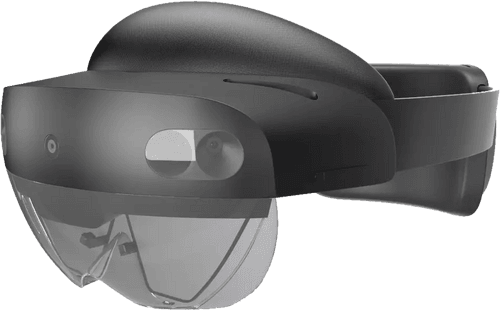
\includegraphics[width=10cm]{img/microsofthololens2.png}
  \caption{Headset Microsoft HoloLens 2.}
  \label{hololens}
\end{figure}	

%\subsubsection{Zobrazovacia technológia}
HoloLens 2 využíva na zobrazovanie obrazu dva priehľadné holografické displeje typu \acrshort{lbs}, každý s rozlíšením 1440x936 pixelov a obnovovaciou frekvenciou
 60 Hz \cite{MicrosoftHoloLensFull}. 
\acrshort{lbs} dokáže poskytnúť široké zorné pole; v spojení s vysokým rozlíšením umožňuje v prostredí používateľa zobraziť hologramy s vysokou úrovňou detailov.

Súčasťou HoloLensu sú taktiež rôzne senzory a kamery, ktoré umožňujú snímať a vyhodnocovať prostredie, v ktorom sa používateľ práve nachádza \cite{AdvancingMRExperience}. 
Dáta o prostredí sú získavané pomocou nasledujúceho vybavenia:
\begin{itemize}
  \item Kamery sledujúce prostredie vo viditeľnom spektre\footnote{Visible Light Environment Tracking}
  \item Hĺbková kamera
  \item Farebná kamera
  \item Pohybové senzory
  \item Infračervené kamery
  \item Pole mikrofónov  
\end{itemize}

Štvorica kamier sledujúcich prostredie vo viditeľnom spektre snímajú obraz v škále šedej; ich obraz sa používa na sledovanie pohybu hlavy a vytváranie priestorovej mapy.
Hĺbková kamera sníma priestor v dvoch režimoch. Prvý režim sníma priestor rýchlosťou 45 snímkov za sekundu a slúži primárne na zaznamenávanie pohybu rúk; presnú vzdialenosť
dokáže detegovať približne do jedného metra. V druhom režime, ktorý je určený na priestorové mapovanie, je rýchlosť snímania v rozmedzí jeden až päť snímkov za sekundu.
V oboch režimoch však kamera dokáže poskytovať obrázky v infračervenom spektre, ktoré nie sú ovplyvnené ambientným svetlom.
\\\\
\noindent Pohybové senzory, ktoré HoloLens používa, sú nasledovné:
\begin{itemize}
  \item akcelerometer, ktorý sníma zrýchlenie na všetkých osiach,
  \item gyroskop, ktorý slúži na detekciu rotácie, a
  \item magnetometer, ktorý pomáha určiť absolútnu orientáciu.
\end{itemize}
Farebná kamera umožňuje snímať obrázky v rozlíšení 8 megapixelov, alebo natáčať video v rôznych rozlíšeniach. Medzi jej funkcie patrí automatické zaostrovanie, vyváženie bielej,
automatické nastavenie expozície a i. Pomocou tejto kamery je možné zaznamenávať \acrshort{mr} zážitok a zdieľať ho s ostatnými ľuďmi tak, ako ho vidí používateľ 
prostredníctvom funkcie Mixed Reality Capture.

Pomocou infračerevných kamier zabudovaných v headsete je možné sledovať pohyb očí používateľa. Táto funkcia umožňuje detegovať používateľov pohľad a reagovať naň, vďaka čomu 
môže byť \acrshort{mr} zážitok intenzívnejší a interakcia s virtuálnym svetom dokáže byť intuitívnejšia. 
Prostým pohľadom dokáže používateľ presúvať virtuálne objekty, posúvať čítaný text; taktiež je možné sledovať pozornosť používateľa v danom okamihu \cite{EyeTrackingHoloLens}.
Táto funkcia je oproti predchádzajúcej verzii headsetu novinkou.

Prostredníctvom poľa mikrofónov dokáže HoloLens reagovať na hlasové povely, čo v spojení so sledovaním pohybu očí umožňuje efektívne používanie headsetu aj bez použitia rúk.

%\newpage
\subsection{Vývoj aplikácií pre Microsoft HoloLens 2}
Microsoft vývojárom poskytuje \acrshort{mrtk} (\acrlong{mrtk}), čo je multiplatformová knižnica, ktorá významne urýchľuje a zjednodušuje prácu vývojárov pri tvorbe aplikácií
pre umelú realitu. Prostredníctvom tejto knižnice je možné rýchle prototypovanie aplikácií za použitia rôznych \acrshort{ui}/\acrshort{ux} nástrojov, predpripravených šablón 
objektov (napr. tlačidiel) a hotových príkladov aplikácií \cite{valoremreplyWaysMicrosoftMixed}. 

\acrshort{mrtk} je dostupný pre populárny herný engine Unity. Unity je dostupné bezplatne pre osobné použitie, čo robí takýto vývoj prístupný širokému spektru záujemcov.
Programový kód aplikácií vyvíjaných v tomto prostredí je písaný v jazyku C\#. Samostatná verzia \acrshort{mrtk} existuje aj pre nástroj s názvom Unreal Engine. Unreal
Engine sme si zvolili na realizáciu aplikácie tejto diplomovej práce; jeho detailnejšiemu popisu a dôvodom jeho voľby sa budeme venovať v kapitole \todo{cislo kapitoly}.

Okrem HoloLens 2 je podporovaných niekoľko ďalších zariadení, napr. Meta Quest \cite{microsoftWhatMixedReality}. Takztiež sú podporované platformy postavené na platforme
iOS a Android. Jednou z výhod multiplatformovosti je aj jednoduchý prenos aplikácie napísanej pre pôvodnu verziu HoloLens na verziu 2. Rovnako sa dá veľká časť programu
otestovať na jednom zariadení, a na ostatných zariadeniach, s ktorými sa pri vývoji počíta, sa už len dolaďujú špecifické detaily.

Na to, aby dokázal vývojár otestovať svoju aplikáciu, nemusí mať prístup k headsetu ako takému. Nástroj s názvom HoloLens Emulator umožňuje odskúšanie takejto aplikácie 
na počítači, pričom vstupy sú simulované pomocou myši, klávesnice, prípadne ovládača Xbox. Pre použitie v emulátore nie je nutné aplikáciu žiadnym spôsobom upravovať. 
Pohyb v priestore je ovládaný rovnako, ako v typickej počítačovej hre (klávesy W, A, S a D), pohybom myši sa simuluje pohyb rúk a hlavy \cite{microsoftUsingHoloLensEmulator}.

\subsection{Súčasné využitie umelej reality vo vzdelávaní}
Umelá realita sa čoraz viac využíva vo vzdelávaní v oblasti biológie. Imerzívne zážitky, ktoré využívajú ľudské zmysly, sú vo vzdelávaní v oblasti biológie obzvlášť prínosné, 
pretože umožňujú študentom oboznámiť sa s komplexnými biologickými systémami, ktoré nie je ľahké realizovať vo fyzickom svete, ako sú napríklad štruktúry bielkovín alebo bunkové procesy. 
Napríklad \acrshort{vr} platformy, ako sú VRLab Academy, Labster a ClassVR, simulujú biologické a chemické experimenty v prostredí VR, čím zlepšujú zážitok z učenia \cite{turhanBraveNewWorld2022}.

Turhan ďalej tvrdí, že randomizované štúdie ukázali, že stereoskopické 3D nástroje pomáhajú pri učení anatómie a študenti ich prijímajú veľmi pozitívne. Zvyšujúca sa dostupnosť vzdelávacích platforiem 
a nástrojov vo \acrshort{vr} svedčí o jej rastúcej úlohe vo vzdelávaní v oblasti biológie. Využívanie herných mechanizmov v týchto platformách, ako je napríklad VR nástroj Peppy založený na Unity, 
pomáha pri pochopení zložitých biologických štruktúr a procesov. Tieto imerzívne vizualizácie uľahčujú pochopenie abstraktných pojmov, ktoré sú tradične náročné na pochopenie 
prostredníctvom fyzických modelov alebo 2D reprezentácií.

Potenciál VR vo vzdelávaní v oblasti biológie je významný, pretože ponúka nové spôsoby skúmania, experimentovania a pochopenia zložitých biologických údajov a konceptov. S ďalším 
vývojom technológií sa očakáva, že využívanie umelej reality vo vzdelávaní v oblasti biológie sa bude rozširovať a bude ponúkať interaktívnejšie a pútavejšie vzdelávacie skúsenosti.

Pozitívna spätná väzba od študentov a preukázaná účinnosť pri napomáhaní k hlbšiemu pochopeniu biologických systémov ďalej motivujú výskumníkov k vývoju a integrácii týchto technológií 
do vzdelávacích osnov. Prispôsobiteľnosť umelej reality rôznym vzdelávacím kontextom spolu s rýchlym technologickým pokrokom otvára nespočetné možnosti budúcich aplikácií nielen v biológii, 
ale aj v iných oblastiach vedy a vzdelávania.

Malone vo svojej metaanalýze vyhodnocuje vplyvy využitia \acrshort{ar} vo vzdelávaní počas posledných tridsiatich rokov \cite{maloneThreeDecadesAugmented2023}. 
Ústredným zistením tejto štúdie je zistenie, že AR má konzistentný a stredne silný vplyv na výsledky vzdelávania v rôznych vzdelávacích prostrediach. Výskum dokazuje, že účinnosť 
AR presahuje hranice akademických disciplín, demografických charakteristík účastníkov a typov výsledkov vzdelávania. Táto široká použiteľnosť zdôrazňuje úlohu AR ako univerzálneho 
vzdelávacieho nástroja, ktorý dokáže zlepšiť kvalitu vzdelávania v rôznych spektrách výuky.

Štúdia skúma, ako AR ako technologický nástroj ovplyvňuje procesy a výsledky vzdelávania. Syntézou údajov zo širokého spektra štúdií predstavuje holistický pohľad na úlohu AR vo vzdelávaní. 
Výskum sa zaoberá potenciálnymi vplyvmi rôznych faktorov, ako sú disciplína, charakteristiky účastníkov a typ vzdelávacích výsledkov. Dochádza však k záveru, že tieto faktory významne nemenia 
účinnosť AR. Toto zistenie je kľúčové a poukazuje na potenciál AR ako univerzálneho nástroja vo vzdelávaní, ktorý sa môže využívať v rôznych vzdelávacích prostrediach a s rôznymi skupinami učiacich sa.

Štúdia ďalej potvrdzuje potrebu neustáleho výskumu v tejto oblasti a poukazuje na možnosti budúceho skúmania uplatnenia AR vo vzdelávaní. Napriek určitým obmedzeniam poskytujú zistenia silný základ 
pre pochopenie možností AR pri zlepšovaní vzdelávacích procesov a výsledkov. V štúdii sa tiež zdôrazňuje kvalita zahrnutých metaanalýz, pričom sa konštatuje ich všeobecne prijateľná až dobrá kvalita, 
čo prispieva k spoľahlivosti zistení.

\subsection{Miskoncepcie - TODO}
\todo{upratat}
\subsubsection{Bunka ako trojrozmerný objekt}
Vijapurkar uvádza, že problém pri vzdelávaní študentov, pokiaľ ide o presnú vizualizáciu buniek, vyplýva z ich hlboko zakorenenej mylnej predstavy o bunkách ako dvojrozmerných 
štruktúrach \cite{vijapurkarWhatCellsReally2014}. Aj keď sú bunky na ilustráciách znázornené ako trojrozmerné, tieto snahy často nepomáhajú študentom vytvoriť si správnu trojrozmernú 
predstavu. Tento problém sa neobmedzuje len na nedostatok trojrozmernosti v mentálnych modeloch študentov; ide aj o ich neschopnosť vnímať bunky ako dynamické, funkčné jednotky života, 
čo je v biológii kľúčový koncept.

Jedným z kľúčových faktorov, ktoré prispievajú k tomuto problému, je charakter ilustrácií v učebniciach. Učebnice a vzdelávacie materiály sa zvyčajne vo veľkej miere spoliehajú na 2D 
projekcie 3D objektov. Hoci tieto ilustrácie majú znázorňovať trojrozmerné štruktúry, často to študentom účinne nesprostredkujú. Je to preto, že prevod 2D projekcie na 3D koncept je 
zložitá kognitívna úloha, najmä pre mladších študentov. Problém ešte znásobuje skutočnosť, že bunky, ktoré sú mikroskopické, sú mimo rozsahu bežnej ľudskej skúsenosti, čo sťažuje študentom 
pochopiť a predstaviť si ich skutočnú povahu a rozsah.

Štúdia zdôraznila, že aj keď sa študentom ukážu skutočné fotografie buniek, ktoré ich zobrazujú ako 3D objekty, ich už existujúce 2D mentálne modely môžu narušiť ich interpretáciu týchto 
obrázkov. Táto nesprávna interpretácia naznačuje, že problém nespočíva len v spôsobe zobrazovania buniek, ale aj v tom, ako sa študenti učia chápať tieto zobrazenia.

Ďalej Vijapurkar spomína, že keď sa študenti v triede venovali vytváraniu fyzických modelov buniek, ich prvé pokusy stále odrážali 2D perspektívu, pričom modely mali podhodnotený 
tretí rozmer. Ako však vyučovanie postupovalo so zameraním na spochybňovanie a pretváranie ich mentálnych modelov, následné modely študentov vykazovali výrazné zlepšenie v zobrazovaní 
3D povahy buniek. Tento prechod podčiarkuje význam aktívnych, praktických skúseností pri učení sa, ktoré pomáhajú študentom vytvárať presné mentálne modely.

Pretrvávajúca povaha tohto problému s 2D vizualizáciou naznačuje, že by mohli byť potrebné interaktívnejšie a imerzívnejšie vyučovacie metódy. Tu môžu zohrávať kľúčovú úlohu počítačové 
3D modely a aplikácie zmiešanej reality (\acrshort{mr}). Tieto pokročilé technologické nástroje môžu študentom poskytnúť interaktívne trojrozmerné reprezentácie buniek, ktoré im umožnia preskúmať a 
pochopiť zložité štruktúry intuitívnejším a pútavejším spôsobom. Najmä aplikácie \acrshort{mr} ponúkajú imerzívny zážitok, ktorý môže preklenúť rozdiely medzi 2D reprezentáciami a 3D realitou a pomôcť 
študentom lepšie pochopiť koncept buniek ako dynamických trojrozmerných štruktúr. Kombináciou vizuálnych, sluchových a hmatových podnetov môže \acrshort{mr} vytvoriť komplexnejší vzdelávací zážitok, 
ktorý môže účinne riešiť a korigovať hlboko zakorenené mylné predstavy študentov o povahe buniek.

Na záver možno konštatovať, že hoci tradičné metódy zobrazovania buniek v 3D nestačia na to, aby pomohli študentom vytvoriť si presné vizuálne predstavy, začlenenie moderných technológií, 
ako sú počítačové 3D modely a aplikácie zmiešanej reality, by mohlo poskytnúť účinnejšie riešenie pri pretváraní študentských predstáv o bunkách ako komplexných, dynamických a trojrozmerných štruktúrach.

\subsubsection{Nepresnosti pri výuke problematiky nervových vzruchov}
Odomova štúdia \cite{odomActionPotentialsBiology1993} identifikuje osem kľúčových konceptov týkajúcich sa akčného potenciálu a hodnotí ich presnosť a obsiahnutie v šiestich 
stredoškolských učebniciach biológie. Zistenia odhaľujú rôznorodosť rozsahu pokrytia konceptov súvisiacich s nervovým vzruchom, pričom niektoré učebnice poskytujú komplexnejšie 
a presnejšie informácie ako iné. Uvádza sa, že väčšina učebníc prezentuje pojmy prostredníctvom textu alebo ilustrácií, pričom chýbajú praktické úlohy v laboratóriu. 

V dokumente sa tiež uvádzajú konkrétne miskoncepcie zistené v vyhodnocovaných učebniciach, ako napríklad nepresnosti týkajúce sa úlohy sodíkovo-draslíkovej pumpy pri repolarizácii 
a zavádzajúce analógie porovnávajúce nervové vzruchy s elektrickým prúdom v drôtoch. 

Okrem toho štúdia ďalej zdôrazňuje nevyhnutnosť presného a komplexného pokrytia problematiky nervových vzruchov v učebniciach biológie, najmä vzhľadom na zásadnú úlohu neurobiológie 
pri porozumení biológie človeka. V článku sa tiež pojednáva o vývoji modelov a počítačových simulácií na pomoc pri výučbe pojmov akčného potenciálu, pričom sa poukazuje na potrebu 
praktických skúseností študentov na pochopenie týchto abstraktných konceptov. 



\subsection{Procesy na nervových vláknach}

Na nervových vláknach prebiehajú dva procesy: 
\begin{itemize}
  \item vzrušenie (excitácia), teda vznik nervového vzruchu
  \item vedenie nervového vzruchu (kondukcia, šírenie, propagácia)
\end{itemize}

\subsubsection{Vzrušenie nervového vlákna}

Nervový vzruch je stereotypný sled depolarizácie a repolarizácie vzrušivej membrány nervového vlákna, ktorý vzniká spontánne vždy, keď depolarizácia dosiahne úroveň prahovej depolarizácie.
Nervový vzruch sa tiež nazýva akčný potenciál. Ak nervové vlákno dráždime slabými podnetmi, voltáž membránového potenciálu sa síce zníži, ale táto depolarizácia nedosiahne úroveň prahovej
depolarizácie a akčný potenciál nevznikne. Takéto podnety nazývame podprahovými podnetmi. Až prahový podnet depolarizuje membránu k prahovej úrovni a zrodí sa akčný potenciál.

\subsubsection{Vedenie akčného potenciálu}

Sú dva typy vedenia akčného potenciálu - vedenie po nemyelinizovanom a vedenie po myelinizovanom nervovom vlákne.

\paragraph{Vedenie na nemyelinizovanom vlákne.} 
Vzrušený úsek vlákna má obrátenú polaritu - povrch je elektronegatívny a vnútro elektropozitívne. Zo susedného normálne polarizovaného miesta (povrch pozitívny, vnútro negatívne) prechádzajú
kladné náboje k vzrušenému elektronegatívnemu miestu a potom spolu s Na\textsuperscript{+} vnikajú dovnútra a tam idú niekoľko milimetrov opačným smerom. Týmto pohybom nábojov sa oslabuje 
elektropozitivita susedného miesta zvonku a posilňuje zvnútra. Oslabovanie elektropozitivity znamená oslabovanie polarizácie, pokles membránového potenciálu až k úrovni prahovej depolarizácie,
čím sa vyvolá akčný potenciál už na novom mieste. Posun akčného potenciálu je plynulý, no rýchlosť jeho vedenia je relatívne malá.

\paragraph{Vedenie na myelinizovanom vlákne.}
Myelinizované nervové vlákna sú obalené myelínovými obalmi (pošvami). Tie nie sú súvislé, ale prerušované v miestach Ranvierovych zárezov. Iba v týchto miestach je vodivá membrána v styku s mimobunkovou 
tekutinou a teda len v týchto miestach je polarizovaná. Ak sa akčný potenciál práve nachádza v jednom Ranvierovom záreze, povrch membrány je tu elektronegatívny a jej vnútorná strana 
elektropozitívna. Opäť je tu prítomný fenomén oslabovania elektropozitivity, tentokrát ale najbližšieho Ranvierovho zárezu, ktorý môže byť vzdialený jeden až dva milimetre. Aj tu platí, že ak
depolarizácia membrány v susednom záreze dosiahne prahovú hodnotu, zrodí sa v ňom nervový vzruch. Ten sa naň teda presunul skokom. Tento typ vedenia možno charakterizovať týmito vlastnosťami:

\begin{itemize}
  \item ióny nemôžu prestupovať cez myelínový obal, len cez obnaženú membránu v Ranvierovom záreze,
  \item nervový vzruch ,,skáče'' zo zárezu do zárezu, preto hovoríme o saltatórnom vedení (,,vedení skokom''),
  \item dĺžka jedného myelinizovaného úseku (internódium) závisí od priemeru vlákna - čím je hrubšie, tým je myelinizovaný úsek (a teda i skok) dlhší,
  \item čas jedného skoku nezávisí od dĺžky internódia, je rovnaký pri dlhých i krátkych internódiach. Ak sú dlhšie (na hrubších vláknach), ich počet je menší a teda i počet skokov na jednotku dĺžky vlákna bude menší. To zvyšuje rýchlosť vedenia a následne napr. reflexný a reakčný čas,
  \item iónové prúdy sú obmedzené len na Ranvierove zárezy, teda menej iónov prechádza na jednotku povrchu nervového vlákna a sekundárne menej energie treba na udržovanie a obnovu koncentračných rozdielov Na\textsuperscript{+} a K\textsuperscript{+} v mimobunkovej a vnútrobunkovej tekutine.
\end{itemize}

Saltatórne vedenie je takto nielen veľmi rýchle, ale i veľmi hospodárne. Je obdivuhodne dômyselnou inováciou informačných tokov v živých systémoch \cite{bederFyziologiaCloveka2005}.

\subsubsection{Iónové zmeny počas vedenia akčného potenciálu}

Zmenou polarizácie membrány oproti pokojovým podmienkam sa výrazne mení jej priepustnosť pre ióny Na\textsuperscript{+} - pri depolarizácii sa priepustnosť pre Na\textsuperscript{+} zvyšuje, 
pri hyperpolarizácii sa znižuje. Zmena priepustnosti pre Na\textsuperscript{+} sa uskutočňuje prostredníctvom napäťovo závislých sodíkových kanálov. Depolarizácia membrány vyvoláva aj 
otváranie pomalých draslíkových kanálov. 

Pri podprahových stimuláciách , na ktoré reaguje membrána iba miestnym podráždením, t.j. stupňovaným potenciálom, výstup K\textsubscript{+} prevažuje nad vstupom Na\textsuperscript{+}. 
Úroveň depolarizácie sa už teda nemôže ďalej zvyšovať a membrána sa vracia do pokojového stavu. Ak má však podnet prahovú úroveň, resp. stupeň depolarizácie membrány dosahuje spúšťaciu úroveň
-55 mV, sodíkové kanály sa prudko otvárajú, priepustnosť pre Na\textsuperscript{+} sa niekoľkostonásobne zvyšuje a vstup Na\textsuperscript{+} v smere koncentračného aj elektrického gradientu
mnohonásobne prevyšuje výstup K\textsuperscript{+}. Tieto rýchle zmeny iónového rozloženia na membráne majú za následok prudkú depolarizáciu až transpolarizáciu membrány, korešpondujúcu so vzostupným
ramenom hrotového potenciálu.

Sodíkové kanály sa aj napriek pretrvávajúcej depolarizácii veľmi rýchlo inaktivujú, čo sprevádza rýchle znižovanie priepustnosti membrány pre ióny Na\textsuperscript{+}. Táto zmena je spoločne 
so zvýšením permeability pre ióny K\textsuperscript{+} zodpovedná za rýchly návrat hrotového potenciálu na pokojovú úroveň. Pri následnej hyperpolarizácii už dosahuje priepustnosť membrány pre 
Na\textsuperscript{+} východiskovú úroveň , kým pre K\textsuperscript{+} zostáva zvýšená nad pokojový stav.

Na následnej hyperpolarizácii (pozitívny následný potenciál) sa zúčastňuje aj elektrogénny efekt sodíkovo-draslíkovej pumpy, ktorá participuje i na obnovení pôvodného rozloženia iónov.
Intracelulárnemu hromadeniu Na\textsuperscript{+} a zvyšovaniu extracelulárnej koncentrácie K\textsuperscript{+} zabraňuje trvalé pôsobenie sodíkovo-draslíkovej pumpy ktorá udržuje stály pokojový 
membránový potenciál. \cite{javorkaLekarskaFyziologiaUcebnica2001}

\todo{kapitola} kapitola 

Na realizáciu aplikácie boli použité nástroje Blender a Unreal Engine. Blender je slobodný a otvorený \todo{FOSS} softvér pre prácu s trojrozmernou grafikou. Používa sa na 3D modelovanie,
animáciu, tvorbu vizuálnych efektov, a pod. Unreal Engine je herný engine vyvíjaný spoločnosťou Epic Games. Pôvodne bol určený pre vývoj FPS hier \todo{FPS}, no dnes má širokú škálu použitia
od vývoja najrôznejších herných titulov a tvorbu filmových efektov až po architektonické vizualizácie a tvorbu aplikácií určených pre virtuálnu, rozšírenú a zmiešanú realitu.

Model neurónu sme si pripravili v Blenderi. Prvým krokom bolo vytvorenie nového projektu voľbou \texttt{General} v úvodnom dialógu po spustení Blendera. Štandardne sú v novom projekte 
umiestnené vzorové objekty (kocka, zdroj svetla a kamera). Tieto neboli pre naše použitie potrebné, odstránili sme ich. Do projektu sme pridali nový objekt typu \texttt{UV Sphere}, 
ktorý nám poslúžil ako základ pre ďalšie tvarovanie pomocou techniky zvanej sculpting. 

Sculpting v digitálnom modelovaní je podobný tradičnému sochárstvu, kde 3D grafik formuje a upravuje digitálny objekt ručne. Tento proces zahŕňa použitie
rôznych nástrojov a techník, ako je napríklad \emph{Snake hook} slúžiaci na vyťahovanie dlhých, tiahlych tvarov, \emph{Inflate} pre dodanie objemu alebo zväčšenie špecifických oblastí modelu,
\emph{Crease} pre vytváranie ostrých línií a zárezov, alebo \emph{Smooth} pre vyhladzovanie povrchov. Tento prístup je obzvlášť vhodný pre modelovanie prírodných objektov, ako sú neuróny, 
ktoré majú komplexnú a nepravidelnú štruktúru. Na rozdiel od iných metód modelovania, kde sa kladie dôraz na geometrickú presnosť a dodržiavanie technických výkresov, sculpting umožňuje 
väčšiu flexibilitu a intuitívnosť. Týmto spôsobom sme mohli efektívne zachytiť jedinečné a zložité tvary neurónu, čo by bolo pri použití iných modelovacích techník náročnejšie. 
Táto metóda poskytuje slobodu v tvorbe a umožňuje dosiahnuť vyššiu úroveň vizuálnej autenticity, čo je kľúčové pre správne reprezentovanie organických štruktúr, akými sú neuróny.

\texttt{UV Sphere}, ktorý sme v predošlom kroku vytvorili, sme použili pre vytvorenie tela neurónu. To zahŕňalo formovanie základnej štruktúry neurónu, kde sme sa zamerali na vytvorenie
výbežkov, ktoré predstavovali základ pre dendrity. Následne sme tento základ rozvetvili do komplexnejšej stromovej štruktúry.

Po prepnutí sa do režimu \emph{sculpting} sme v pravom paneli zaškrtli voľbu \texttt{Dyntopo}, čo je skratka pre \emph{Dynamic topology}. Táto funkcia Blenderu umožňnuje dynamickú zmenu
topológie pri sculptingových úpravách. Flexibilita pri práci, ktorá sa vykonáva pomocou sculptingu, by bola významne obmedzená pevne definovaným počtom polygónov. \emph{Dyntopo} tento problém
rieši tým, že automaticky pridáva alebo odoberá v oblastiach, s ktorými sa pracuje. To znamená, že pri používaní rôznych sculptingových nástrojov sa topológia mení automaticky podľa potreby.
Pre vytváranie výbežkov sme použili nástroje \emph{Snake hook} a \emph{Elastic deform}, ktoré nám umožnili presne a flexibilne modelovať ich dlhé a tenké štruktúry. Po vytvorení základných výbežkov
sme prešli k detailnejšej práci na stromových štruktúrach na koncoch výbežkov. Na ich tvorbu sme využili rovnaké nástroje, pričom sme dbali na to, aby rozloženie a hustota vetiev reflektovala
vyobrazenie neurónu v dostupných materiáloch. \todo{vzorove obrazky}

Ďalším krokom bolo vymodelovanie axónu. Ako základ axónu sme použili Bézierovú krivku. Bézierová krivka je parametrická krivka umožňujúca tvorbu hladkých zakrivených tvarov, pričom výsledný tvar je
jednoducho modifikovateľný pomocou riadiacich bodov. Do projektu sme vložili novú Bézierovu krivku. Jej umiestnenie v priestore sme volili tak, aby jeden koniec zasahoval do tela neurónu 
a druhý koniec sa nachádzal v adekvátnej vzdialenosti - v mieste, kde sme mali v úmysle neskôr vytvoriť zakončenia axónu. Po vhodnom vytvarovaní krivky sme v záložke \texttt{Object Data Properties}
v sekcii \texttt{Geometry} $\rightarrow$ \texttt{Bevel} nastavili parameter \texttt{Depth} tak, aby táto krivka nadobudla adekvátny objem. Následne sme túto krivku prekonvertovali na mesh, aby 
sme ju neskôr mohli detailnejšie tvarovať pomocou sculptingu. \todo{Popisat join?}
Pomocou nástroja \emph{Inflate} sme zväčšili objem meshu v oblasti konca krivky a tiež v mieste, kde sa krivka spája s telom neurónu. 

Poslednou časťou neurónu, ktorú sme potrebovali zahrnúť do modelu, bola myelínová pošva. Ako jej základ poslúžil objekt typu \texttt{Cylinder}, ktorý sme viacnásobným použitím nástroja \emph{Bevel} postupne
upravili do zodpovedajúceho tvaru pripomínajúceho súdok. Tento objekt sme následne zduplikovali celkom desaťkrát a jednotlivé kópie sme umiestnili za sebou na vymodelovaný axón tak, aby medzi 
nimi boli medzery reprezentujúce Ranvierove zárezy.